%
% Main document
% ===========================================================================
% This is part of the document "Project documentation template".
% Authors: brd3, kaa1
%

%---------------------------------------------------------------------------
\documentclass[
	a4paper,					% paper format
	10pt,							% fontsize
	twoside,					% double-sided
	openright,				% begin new chapter on right side
	notitlepage,			% use no standard title page
	parskip=half,			% set paragraph skip to half of a line
]{scrreprt}					% KOMA-script report
%---------------------------------------------------------------------------

\raggedbottom
\KOMAoptions{cleardoublepage=plain}			% Add header and footer on blank pages


% Load Standard Packages:
%---------------------------------------------------------------------------
\usepackage[standard-baselineskips]{cmbright}

\usepackage[ngerman,english]{babel}										% english hyphenation
%\usepackage[latin1]{inputenc}  							% Unix/Linux - load extended character set (ISO 8859-1)
\usepackage[ansinew]{inputenc}  							% Windows - load extended character set (ISO 8859-1)
\usepackage[T1]{fontenc}											% hyphenation of words with �,� and �
\usepackage{textcomp}													% additional symbols
\usepackage{ae}																% better resolution of Type1-Fonts 
\usepackage{fancyhdr}													% simple manipulation of header and footer 
\usepackage{etoolbox}													% color manipulation of header and footer
\usepackage{graphicx}                      		% integration of images
\usepackage{float}														% floating objects
\usepackage{caption}													% for captions of figures and tables
\usepackage{booktabs}													% package for nicer tables
\usepackage{tocvsec2}													% provides means of controlling the sectional numbering
%---------------------------------------------------------------------------

% Load Math Packages
%---------------------------------------------------------------------------
\usepackage{amsmath}                    	   	% various features to facilitate writing math formulas
\usepackage{amsthm}                       	 	% enhanced version of latex's newtheorem
\usepackage{amsfonts}                      		% set of miscellaneous TeX fonts that augment the standard CM
\usepackage{amssymb}													% mathematical special characters
\usepackage{exscale}													% mathematical size corresponds to textsize
%---------------------------------------------------------------------------

% Package to facilitate placement of boxes at absolute positions
%---------------------------------------------------------------------------
\usepackage[absolute]{textpos}
\setlength{\TPHorizModule}{1mm}
\setlength{\TPVertModule}{1mm}
%---------------------------------------------------------------------------					
			
% Definition of Colors
%---------------------------------------------------------------------------
\RequirePackage{color}                          % Color (not xcolor!)
\definecolor{linkblue}{rgb}{0,0,0.8}            % Standard
\definecolor{darkblue}{rgb}{0,0.08,0.45}        % Dark blue
\definecolor{bfhgrey}{rgb}{0.41,0.49,0.57}      % BFH grey
%\definecolor{linkcolor}{rgb}{0,0,0.8}     			% Blue for the web- and cd-version!
\definecolor{linkcolor}{rgb}{0,0,0}        			% Black for the print-version!
%---------------------------------------------------------------------------

% Hyperref Package (Create links in a pdf)
%---------------------------------------------------------------------------
\usepackage[
	pdftex,ngerman,bookmarks,plainpages=false,pdfpagelabels,
	backref = {false},										% No index backreference
	colorlinks = {true},                  % Color links in a PDF
	hypertexnames = {true},               % no failures "same page(i)"
	bookmarksopen = {true},               % opens the bar on the left side
	bookmarksopenlevel = {0},             % depth of opened bookmarks
	pdftitle = {Template f�r Bachelor Thesis},	   	% PDF-property
	pdfauthor = {brd3},        					  % PDF-property
	pdfsubject = {LaTeX Template},        % PDF-property
	linkcolor = {linkcolor},              % Color of Links
	citecolor = {linkcolor},              % Color of Cite-Links
	urlcolor = {linkcolor},               % Color of URLs
]{hyperref}
%---------------------------------------------------------------------------

% Set up page dimension
%---------------------------------------------------------------------------
\usepackage{geometry}
\geometry{
	a4paper,
	left=28mm,
	right=15mm,
	top=30mm,
	headheight=20mm,
	headsep=10mm,
	textheight=242mm,
	footskip=15mm
}
%---------------------------------------------------------------------------

% Makeindex Package
%---------------------------------------------------------------------------
\usepackage{makeidx}                         		% To produce index
\makeindex                                    	% Index-Initialisation
%---------------------------------------------------------------------------

% Glossary Package
%---------------------------------------------------------------------------
% the glossaries package uses makeindex
% if you use TeXnicCenter do the following steps:
%  - Goto "Ausgabeprofile definieren" (ctrl + F7)
%  - Select the profile "LaTeX => PDF"
%  - Add in register "Nachbearbeitung" a new "Postprozessoren" point named Glossar
%  - Select makeindex.exe in the field "Anwendung" ( ..\MiKTeX x.x\miktex\bin\makeindex.exe )
%  - Add this [ -s "%tm.ist" -t "%tm.glg" -o "%tm.gls" "%tm.glo" ] in the field "Argumente"
%
% for futher informations go to http://ewus.de/tipp-1029.html
%---------------------------------------------------------------------------
\usepackage[nonumberlist]{glossaries}
\makeglossaries

\newglossaryentry{BibTeX}{name={BibTeX},description={Program for the creation of 	bibliographical references and directories in \TeX or \LaTeX documents}}
\newglossaryentry{Index}{name={Index},description={Index with keywords from text}}



%---------------------------------------------------------------------------

% Intro:
%---------------------------------------------------------------------------
\begin{document}                              	% Start Document
\settocdepth{section}														% Set depth of toc
\pagenumbering{roman}														
%---------------------------------------------------------------------------

\providecommand{\heading}{Title of Thesis}		%  Insert Title of Thesis here					% Titel der Arbeit aus Datei titel.tex lesen
\providecommand{\versionnumber}{1.2}			%  Hier die aktuelle Versionsnummer eingeben
\providecommand{\versiondate}{07.02.2014}		%  Hier das Datum der aktuellen Version eingeben				% Versionsnummer und -datum aus Datei version.tex lesen

% Set up header and footer
%---------------------------------------------------------------------------
\makeatletter
\patchcmd{\@fancyhead}{\rlap}{\color{bfhgrey}\rlap}{}{}		% new color of header
\patchcmd{\@fancyfoot}{\rlap}{\color{bfhgrey}\rlap}{}{}		% new color of footer
\makeatother

\fancyhf{}																		% clean all fields
\fancypagestyle{plain}{												% new definition of plain style	
	\fancyfoot[OR,EL]{\footnotesize \thepage} 	% footer right part --> page number
	\fancyfoot[OL,ER]{\footnotesize \heading, Version \versionnumber, \versiondate}	% footer even page left part 
}

\renewcommand{\chaptermark}[1]{\markboth{\thechapter.  #1}{}}
\renewcommand{\headrulewidth}{0pt}				% no header stripline
\renewcommand{\footrulewidth}{0pt} 				% no bottom stripline

\pagestyle{plain}
%---------------------------------------------------------------------------


% Title Page and Abstract
%---------------------------------------------------------------------------
%%
% Project documentation template
% ===========================================================================
% This is part of the document "Project documentation template".
% Authors: brd3, kaa1
%

\begin{titlepage}


% BFH-Logo absolute placed at (28,12) on A4 and picture (16:9 or 15cm x 8.5cm)
% Actually not a realy satisfactory solution but working.
%---------------------------------------------------------------------------
\setlength{\unitlength}{1mm}
\begin{textblock}{20}[0,0](28,12)
	
\includegraphics[scale=1.0]{images/BFH_Logo_B.png}
\end{textblock}

% Institution / titel / subtitel / authors / experts:
%---------------------------------------------------------------------------
\begin{flushleft}

\vspace*{21mm}

\fontsize{26pt}{40pt}\selectfont 
\heading				\\							% Read heading from file leader/title.tex
\vspace{2mm}

\fontsize{16pt}{24pt}\selectfont\vspace{0.3em}
Place your subheading here 			\\				% Insert subheading
\vspace{5mm}

\fontsize{10pt}{12pt}\selectfont
\textbf{Description of thesis (semester- / Bachelor thesis / etc.)} \\		% Insert text
\vspace{7mm}

% Abstract (eingeben):
%---------------------------------------------------------------------------
\begin{textblock}{150}(28,100)
\fontsize{10pt}{12pt}\selectfont
[Insert short text (abstract) if desired] \\ 
This document serves as a template for the compilation of reports according to the guidelines of the BFH. The template is written in LATEX and supports the automatic writing of various directories, references, indexing and glossaries. This small text is a summary of this document with a length of 4 to max. 8 lines. \\ 
The cover picture may be turned on or off in the lines 157/158 of the file template.tex.
\end{textblock}

\begin{textblock}{150}(28,225)
\fontsize{10pt}{17pt}\selectfont
\begin{tabbing}
xxxxxxxxxxxxxxx\=xxxxxxxxxxxxxxxxxxxxxxxxxxxxxxxxxxxxxxxxxxxxxxx \kill
Degree course:	\> [z.B. Electrical and Communication Engineering]	\\		% insert name of degree course
Authors:		\> [Test Peter, M\"uster R\"os\"a]		\\					% insert names
Tutor:	\> [Dr.~Xxxx Xxxx, Dr.~Yyyy Yyyy]		\\							% insert names
Constituent:	\> [Wwwww AG]					\\							% insert names
Experts:		\> [Dr.~Zzzz Zzzz]				\\							% insert names
Date:			\> \versiondate					\\							% read from file leader/version.tex
\end{tabbing}

\end{textblock}
\end{flushleft}

\begin{textblock}{150}(28,280)
\noindent 
\color{bfhgrey}\fontsize{9pt}{10pt}\selectfont
Berner Fachhochschule | Haute \'ecole sp\'ecialis\'ee bernoise | Bern University of Applied Sciences
\color{black}\selectfont
\end{textblock}


\end{titlepage}

%
% ===========================================================================
% EOF
%
		% activate for frontpage without picture
%
% Project documentation template
% ===========================================================================
% This is part of the document "Project documentation template".
% Authors: brd3, kaa1
%

\begin{titlepage}


% BFH-Logo absolute placed at (28,12) on A4 and picture (16:9 or 15cm x 8.5cm)
% Actually not a realy satisfactory solution but working.
%---------------------------------------------------------------------------
\setlength{\unitlength}{1mm}
\begin{textblock}{20}[0,0](28,12)
	
\includegraphics[scale=1.0]{images/BFH_Logo_B.png}
\end{textblock}

\begin{textblock}{154}(28,48)
	\begin{picture}(150,2)
		\put(0,0){\color{bfhgrey}\rule{150mm}{2mm}}
	\end{picture}
\end{textblock}

\begin{textblock}{154}[0,0](28,51)
	\begin{figure}
	\centering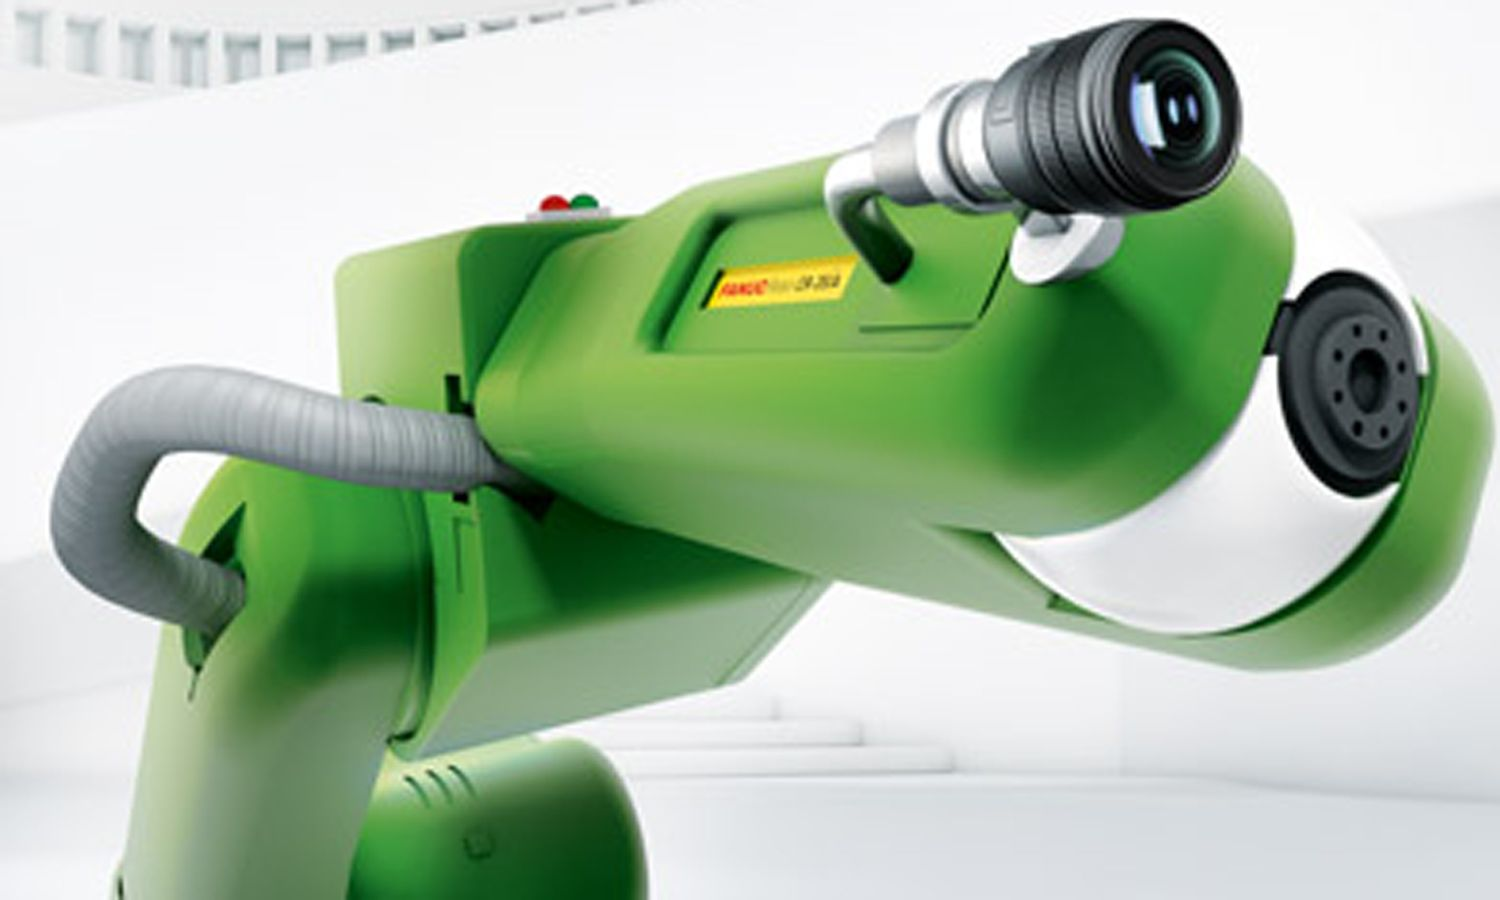
\includegraphics[scale=0.26]{images/fanuc_close.jpg}			% define cover picture
	\captionsetup{textformat=empty,labelformat=blank}
	\caption{Frontpage Picture \cite{fig:frontpage}}
	\end{figure}
\end{textblock}

\begin{textblock}{154}(28,133)
	\begin{picture}(150,2)
		\put(0,0){\color{bfhgrey}\rule{150mm}{2mm}}
	\end{picture}
\end{textblock}
\color{black}

% Institution / titel / subtitel / authors / experts:
%---------------------------------------------------------------------------
\begin{flushleft}

\vspace*{115mm}

\fontsize{26pt}{28pt}\selectfont 
\heading				\\							% Read heading from file leader/title.tex
\vspace{2mm}

\fontsize{16pt}{20pt}\selectfont\vspace{0.3em}
Preliminary Studies of Bachelor Thesis Rob195		\\				% Insert subheading
\vspace{5mm}

%\fontsize{10pt}{12pt}\selectfont
%\textbf{Description of thesis (semester- / Bachelor thesis / etc.)} \\		% Insert text
%\vspace{3mm}

% Abstract (eingeben):
%---------------------------------------------------------------------------
%\begin{textblock}{150}(28,190)
%\fontsize{10pt}{12pt}\selectfont
%[Insert short text (abstract) if desired] \\ 
%This document serves as a template for the compilation of reports according to the guidelines of the BFH. The template is written in LATEX and supports the automatic writing of various directories, references, indexing and glossaries. This small text is a summary of this document with a length of 4 to max. 8 lines. \\ 
%The cover picture may be turned on or off in the lines 157/158 of the file template.tex.
%\end{textblock}

\begin{textblock}{150}(28,225)
\fontsize{10pt}{17pt}\selectfont
\begin{tabbing}
	xxxxxxxxxxxxxxx\=xxxxxxxxxxxxxxxxxxxxxxxxxxxxxxxxxxxxxxxxxxxxxxx \kill
	Degree course:	\> Micro and Medical Technologies	\\		% insert name of degree course
	Author:		\> Aeschlimann Dario		\\					% insert names
	Tutors:	\> Rochat Sarah, Gruener Gabriel		\\							% insert names
	Constituent:	\> AHB Biel					\\							% insert names
	Experts:		\> Aigner Nikita				\\							% insert names
	Date:			\> \versiondate					\\							% read from file leader/version.tex
\end{tabbing}

\end{textblock}
\end{flushleft}

\begin{textblock}{150}(28,280)
\noindent 
\color{bfhgrey}\fontsize{9pt}{10pt}\selectfont
Berner Fachhochschule | Haute \'ecole sp\'ecialis\'ee bernoise | Bern University of Applied Sciences
\color{black}\selectfont
\end{textblock}


\end{titlepage}

%
% ===========================================================================
% EOF
%
		% activate for frontpage with picture
% Control of versions :
% -----------------------------------------------
\newpage
\begin{textblock}{180}(15,150)
\color{black}
\begin{huge}
Versions
\end{huge}
\vspace{10mm}

\fontsize{10pt}{18pt}\selectfont
\begin{tabbing}
xxxxxxxxxxx\=xxxxxxxxxxxxxxx\=xxxxxxxxxxxxxx\=xxxxxxxxxxxxxxxxxxxxxxxxxxxxxxxxxxxxxxxxxxxxxxx \kill
Version	\> Date	\> Status			\> Remarks		\\
0.1	\> 01.08.2013	\> Draft		\> Lorem ipsum dolor sit amet	\\	
0.2	\> 21.08.2013	\> Draft		\> Phasellus scelerisque	\\ 
0.3	\> 02.09.2013	\> Draft		\> Donec eget aliquam urna. Lorem ipsum dolor sit amet	\\ 
1.0	\> 26.01.2014	\> Final		\> Lorem ipsum dolor sit ametPhasellus scelerisque, leo sed iaculis ornare 	\\ 
1.1	\> 31.01.2014	\> Correction	\> Layout changed	\\
1.2	\> 07.02.2014	\> Addition		\> Chapter 1.1 extended	\\
\end{tabbing}

\end{textblock}

\cleardoubleemptypage
\setcounter{page}{1}
\cleardoublepage
\phantomsection 
\addcontentsline{toc}{chapter}{Management Summary}
\chapter*{Management Summary}
\label{chap:managementSummary}

Lorem ipsum dolor sit amet, consectetur adipiscing elit. Phasellus scelerisque, leo sed iaculis ornare, mi leo semper urna, ac elementum libero est at risus. Donec eget aliquam urna. Lorem ipsum dolor sit amet, consectetur adipiscing elit. Nunc fermentum nunc sollicitudin leo porttitor volutpat. Duis ac enim lectus, quis malesuada lectus. Aenean vestibulum suscipit justo, in suscipit augue venenatis a. Donec interdum nibh ligula. Aliquam vitae dui a odio cursus interdum quis vitae mi. Phasellus ornare tortor fringilla velit accumsan quis tincidunt magna eleifend. Praesent nisl nibh, cursus in mattis ac, ultrices ac nulla. Nulla ante urna, aliquet eu tempus ut, feugiat id nisl. Nunc sit amet mauris vitae turpis scelerisque mattis et sed metus. Aliquam interdum congue odio, sed semper elit ullamcorper vitae. Morbi orci elit, feugiat vel hendrerit nec, sollicitudin non massa. Quisque lacus metus, vulputate id ullamcorper id, consequat eget orci \nocite{kopka:band1} \nocite{Marti06}. 

\cleardoubleemptypage
%---------------------------------------------------------------------------

% Table of contents
%---------------------------------------------------------------------------
\tableofcontents
\cleardoublepage
%---------------------------------------------------------------------------

% Main part:
%---------------------------------------------------------------------------
\pagenumbering{arabic}

\chapter{Introduction}
\label{chap:introduction}
\setstretch{1.5}
Collaborative robots are meant to be flexible and easy to be reprogrammed so that they can be used efficiently in the modern industrial environment. One of the most important aspects for collaborative robots is safety. The robot shall not cause any harm to people or material. 
Currently there are three different types \cite{robotiq}  how the workspace of robots is monitored and protected from collisions:

\begin{itemize}
	\item Safety monitored stop: Scanners detect humans and objects inside the workspace of the robot and force a stop of any robot motion. This means the robot is not collaborative.
	\item Speed and separation monitoring: Scanners detect humans and objects inside certain areas around the robot and adjust the speed of the robot when the human comes closer to the robot. This leads to a stop of any robot motion when the human is coming too close to the robot. This is also referred to as cooperative operation.
	\item Power and force limiting: The robot is equipped with force and torque sensor to detect any abnormal forces applied to the robot body. Detecting such a force leads to a stop any robot motion. This type is called collaborative robot.Collisions can also be detected via a  sensitive skin on the robot. The skins can be pressure sensisitive or capacitive. The latter can detect flesh (they typically can not differentiate between a living human and a sausage) within a cm or two next to the skin. 
\end{itemize}
	
%	https://blog.robotiq.com/what-does-collaborative-robot-mean
Robots that rely on force sensors to detect collisions only recognize them and thus stopping any motion when the collision is already taking place. In a collaborative situation, the robot acts within a dynamic workspace and containers with liquids or heavy unstable objects may obstruct the workspace. These objects may be tipped over by the robot without triggering a halt or the halt could be triggered too late based on the force sensors, which could pose a health risk.
In addition, halts caused by the force sensors cause downtime in the production process which leads to higher production costs and longer production times, which companies like to avoid.
The goal of this thesis is to develop a vision system, which detects in real-time any occupied area in the workspace, that means people or objects which are within reach of the robot, and adapts the robots trajectories to avoid any collisions, thus providing an extra layer of safety. This would allow the robot to work in a modifiable workspace together with a human and to adapt his movements according to the human ones \cite{work_desc}. 

GPU-Voxels \cite{GPU-Voxels} is a similar project, that already has a vision system implemented to monitor the surroundings of various robots. It is mostly used in mobile robotics but has some implementations with an collaborative robots.

Commercially available camera based systems like the Pilz SafetyEye \cite{pilz} can recognize changes in the robot environment, however they do not have any capabilities to modify the robot's path.


\chapter{Planning of the preliminary study}
\label{chap:Planning}
\setstretch{1.5}
The first step of this preliminary study was to plan, how to attempt this project. A plan and a timetable had to be created by taking in account the given work specification \cite{work_desc}. These work specifications defined the following goals for the preliminary study.
\setstretch{1.0}
\begin{itemize}
	\item Write specification, test and validation plan.
	\item Perform a literature review.
	\item Select, order and commission parts for test setup.
	\item get familiarized with robot system and Interface.
	\item Integrate a model of the robot in the collision-avoidance software.
	\item Generate a project plan for the thesis.
\end{itemize}
\setstretch{1.5}

The procedure was planned according these goals by giving them a timely order and a duration per task. This plan was implemented in a Gantt chart which is shown in figure \ref{fig:gantt}.
During the execution of this preliminary study, the plan has been adapted to the current state of the work.

As planned, the literature review started right away but takes place over the whole preliminary study, as there will always be some topics that need further research. The research has been done online by using forums and library and program documentations.
Next to the research, the system specification has been one of the first tasks to approach, due to the reason that the specifications build the fundament for the implementation. When system specifications are defined, an according test to validate the system shall be defined and documented. These tests allow to define measurable goals for each implemented specification as the test can be either successful or not. With this information the validation can be carried out. While finishing the test and validation plan, the author must get acquainted with the robot system and its interface.


While getting familiar with the robot system, a decision about the needed hardware components need to be taken. It's important to choose the parts in an early stage of time as they may need some time to be delivered. All components need to be available in week 12 of the project, so that they can be used when the Bachelor Thesis starts.


A big amount of time is planned for the implementation of the robot model. The goal of this implementation is, that the planning of the thesis can be done basing on the progress of this implementation. So the further this implementation is along, the more detailed and realistic the planning of the Thesis can be foreseen.

The Last Week of the preliminary study acts as buffer zone, with reserved time for proofreading and finishing the documentation.
%\section{Timetable}
\begin{landscape}
\begin{figure}[h]
\centering
\begin{ganttchart}[%Specs
y unit title=0.6cm,
y unit chart=0.8cm,
x unit = 0.28cm,
vgrid={*4{black,dotted},*3{red,dashed}},hgrid={black,thin},
title height=1,
newline shortcut=true,
bar label node/.append style={align=left},
%     title/.style={fill=none},
title label font=\bfseries\footnotesize,
bar/.style={fill=blue},
bar height=0.6,
bar top shift=0.2,
%   progress label text={},
group right shift=0,
group top shift=0.8,
group height=.2,
group peaks width={0.4},
inline=false]{1}{77}
%labels
\gantttitle{\textbf{Bachelor Thesis Rob195, Preliminary Studies}}{77}\\  	% title 1
%    \gantttitle[]{Preliminary Studies}{11}     	% title 2
%    \gantttitle[]{Thesis}{11} \\         		% title 3     
\gantttitle{PW1}{7}
\gantttitle{PW2}{7}
\gantttitle{PW3}{7}  
\gantttitle{PW4}{7}  
\gantttitle{PW5}{7}  
\gantttitle{PW6}{7}  
\gantttitle{PW7}{7}  
\gantttitle{PW8}{7}  
\gantttitle{PW9}{7}  
\gantttitle{PW10}{7}  
\gantttitle{PW11}{7}\\
%    dates
\gantttitle{18.2.-24.2.}{7}
\gantttitle{25.2.-03.3.}{7}
\gantttitle{4.3.-10.3.}{7}  
\gantttitle{11.3.-17.3.}{7}  
\gantttitle{18.3.-24.3}{7}  
\gantttitle{25.3.-31.3.}{7}  
\gantttitle{1.4.-7.4.}{7}  
\gantttitle{8.4.-14.4.}{7}  
\gantttitle{15.4.-21.4.}{7}  
\gantttitle{22.4.-28.4.}{7}  
\gantttitle{29.4.-5.5.}{7}\\
%    Week 1
\gantttitle{\rotatebox{90}{M}}{1}
\gantttitle{\rotatebox{90}{T}}{1}  
\gantttitle{\rotatebox{90}{W}}{1}  
\gantttitle{\rotatebox{90}{Th}}{1}  
\gantttitle{\rotatebox{90}{F}}{1}  
\gantttitle{\rotatebox{90}{S}}{1}  
\gantttitle{\rotatebox{90}{Su}}{1}
%    Week 2
 \gantttitle{\rotatebox{90}{M}}{1}
\gantttitle{\rotatebox{90}{T}}{1}  
\gantttitle{\rotatebox{90}{W}}{1}  
\gantttitle{\rotatebox{90}{Th}}{1}  
\gantttitle{\rotatebox{90}{F}}{1}  
\gantttitle{\rotatebox{90}{S}}{1}  
\gantttitle{\rotatebox{90}{Su}}{1} 
%    Week 3
 \gantttitle{\rotatebox{90}{M}}{1}
\gantttitle{\rotatebox{90}{T}}{1}  
\gantttitle{\rotatebox{90}{W}}{1}  
\gantttitle{\rotatebox{90}{Th}}{1}  
\gantttitle{\rotatebox{90}{F}}{1}  
\gantttitle{\rotatebox{90}{S}}{1}  
\gantttitle{\rotatebox{90}{Su}}{1}
%    Week 4
 \gantttitle{\rotatebox{90}{M}}{1}
\gantttitle{\rotatebox{90}{T}}{1}  
\gantttitle{\rotatebox{90}{W}}{1}  
\gantttitle{\rotatebox{90}{Th}}{1}  
\gantttitle{\rotatebox{90}{F}}{1}  
\gantttitle{\rotatebox{90}{S}}{1}  
\gantttitle{\rotatebox{90}{Su}}{1} 
%    Week 5
 \gantttitle{\rotatebox{90}{M}}{1}
\gantttitle{\rotatebox{90}{T}}{1}  
\gantttitle{\rotatebox{90}{W}}{1}  
\gantttitle{\rotatebox{90}{Th}}{1}  
\gantttitle{\rotatebox{90}{F}}{1}  
\gantttitle{\rotatebox{90}{S}}{1}  
\gantttitle{\rotatebox{90}{Su}}{1} 
%    Week 6
 \gantttitle{\rotatebox{90}{M}}{1}
\gantttitle{\rotatebox{90}{T}}{1}  
\gantttitle{\rotatebox{90}{W}}{1}  
\gantttitle{\rotatebox{90}{Th}}{1}  
\gantttitle{\rotatebox{90}{F}}{1}  
\gantttitle{\rotatebox{90}{S}}{1}  
\gantttitle{\rotatebox{90}{Su}}{1} 
%    Week 7
 \gantttitle{\rotatebox{90}{M}}{1}
\gantttitle{\rotatebox{90}{T}}{1}  
\gantttitle{\rotatebox{90}{W}}{1}  
\gantttitle{\rotatebox{90}{Th}}{1}  
\gantttitle{\rotatebox{90}{F}}{1}  
\gantttitle{\rotatebox{90}{S}}{1}  
\gantttitle{\rotatebox{90}{Su}}{1} 
%    Week 8
 \gantttitle{\rotatebox{90}{M}}{1}
\gantttitle{\rotatebox{90}{T}}{1}  
\gantttitle{\rotatebox{90}{W}}{1}  
\gantttitle{\rotatebox{90}{Th}}{1}  
\gantttitle{\rotatebox{90}{F}}{1}  
\gantttitle{\rotatebox{90}{S}}{1}  
\gantttitle{\rotatebox{90}{Su}}{1} 
%    Week 9
 \gantttitle{\rotatebox{90}{M}}{1}
\gantttitle{\rotatebox{90}{T}}{1}  
\gantttitle{\rotatebox{90}{W}}{1}  
\gantttitle{\rotatebox{90}{Th}}{1}  
\gantttitle{\rotatebox{90}{F}}{1}  
\gantttitle{\rotatebox{90}{S}}{1}  
\gantttitle{\rotatebox{90}{Su}}{1} 
%    Week 10
 \gantttitle{\rotatebox{90}{M}}{1}
\gantttitle{\rotatebox{90}{T}}{1}  
\gantttitle{\rotatebox{90}{W}}{1}  
\gantttitle{\rotatebox{90}{Th}}{1}  
\gantttitle{\rotatebox{90}{F}}{1}  
\gantttitle{\rotatebox{90}{S}}{1}  
\gantttitle{\rotatebox{90}{Su}}{1} 
%    Week 11
 \gantttitle{\rotatebox{90}{M}}{1}
\gantttitle{\rotatebox{90}{T}}{1}  
\gantttitle{\rotatebox{90}{W}}{1}  
\gantttitle{\rotatebox{90}{Th}}{1}  
\gantttitle{\rotatebox{90}{F}}{1}  
\gantttitle{\rotatebox{90}{S}}{1}  
\gantttitle{\rotatebox{90}{Su}}{1}                         
%    \gantttitle{TW1}{1}
%    \gantttitle{TW2}{1} 
%    \gantttitle{TW3}{1} 
%    \gantttitle{TW4}{1} 
%    \gantttitle{TW5}{1} 
%    \gantttitle{TW6}{1} 
%    \gantttitle{TW7}{1} 
%    \gantttitle{TW8}{1}   

% Setting group if any
\ganttgroup[inline=false]{Planning}{1}{35}\\ 
\ganttbar[progress=100,inline=false]{System Specification}{1}{23}\\
\ganttbar[progress=100,inline=false]{Test and Validation\ganttalignnewline Plan}{15}{33}\\
\ganttbar[progress=80,inline=false]{Literature Review}{1}{70}\\
\ganttbar[progress=80,inline=false]{Robot System and\ganttalignnewline Interface, Learning}{22}{33}\\
\ganttbar[progress=100,inline=false]{Select comission parts}{28}{33}\\
\ganttmilestone[inline=false]{Ordering comission parts}{33} \\
\ganttgroup[inline=false]{System Implementation}{36}{77}\\ 
\ganttbar[progress=0,inline=false]{Implement Robot Model}{36}{63}\\
\ganttbar[progress=100,inline=false]{Project Plan Thesis}{57}{68}\\

\ganttgroup[inline=false]{Documentation}{1}{77}\\ 
\ganttbar[progress=100,inline=false]{Documentation}{1}{70}\\
\ganttbar[progress=100,inline=false]{Documentation corrections}{71}{75}\\
\ganttmilestone[inline=false]{Hand-In Preliminary Studies}{77} \\

%    \ganttgroup[inline=false]{Thesis}{12}{19} \\ 
%    \ganttbar[progress=2,inline=false]{test1}{10}{19} \\
%    \ganttmilestone[inline=false]{Hand-In Bachelor Thesis}{19} \\
%    \ganttbar[progress=5,inline=false]{test2}{11}{19} \\
%    \ganttmilestone[inline=false]{Milestone 3}{19} \\       

%    \ganttgroup[inline=false]{Group 3}{13}{24} \\ 
%    \ganttbar[progress=90,inline=false]{Task A}{13}{15} \\ 
%    \ganttbar[progress=50,inline=false, bar progress label node/.append style={below left= 10pt and 7pt}]{Task B}{1}{14} \\ \\
%    \ganttbar[progress=30,inline=false]{Task C}{15}{16}\\ 
%    \ganttbar[progress=70,inline=false]{Task D}{18}{20} \\ 
\end{ganttchart}
\caption{Gantt Chart, Preliminary Studies Rob195}
\label{fig:gantt}
\end{figure}
\end{landscape}

\chapter{Instructions}
\label{chap:instructions}

The following table shows some of the most important packages\index{packages} used in the \LaTeX{} template.

\begin{table}[H]
	\centering
		\begin{tabular}{p{0.13\textwidth} p{0.75\textwidth}} \toprule
			\textbf{Package} & \textbf{Function} \\ \midrule
			\texttt{cmbright}\index{cmbright} & sans serif font "Computer Modern Bright", which supports text encodings\index{text encodings} OT1, T1 and TS1, as well as the mathematical signs and AMS symbols \\ \midrule
			\texttt{ae} & provides better resolution fonts in PDF files \\ \midrule
			\texttt{fancyhdr}\index{fancyhdr} & easy adjustment of head- and foot lines \\ \midrule
			\texttt{graphicx}\index{graphicx} & integration of graphics in \LaTeX{} documents \\ \midrule
			\texttt{booktabs}\index{booktabs} & better presentation of tables \\ \midrule
			\texttt{textpos}\index{textpos} & simplified and absolute positioning of boxes on the page \\ \midrule
			\texttt{hyperref}\index{hyperref} & package to complie links into PDF files \\ \midrule
			\texttt{geometry}\index{geometry} & simplified and improved adaptation of the standard type area \\ \midrule
			\texttt{makeidx}\index{makeidx} & simple Index compilation (see section \ref{sec:instructions_index}) \\ \midrule
			\texttt{glossaries}\index{glossaries} & compilation of glossaries (see section \ref{sec:instructions_glossay}) \\ \bottomrule
		\end{tabular}
	\caption{Packages}
	\label{tab:packages}
\end{table}


\section{Subject Indices}
\label{sec:instructions_index}

\LaTeX{} is not able to create an \gls{Index}\index{Index} in the basic configuration. This can be created in \LaTeX{} with the \texttt{makeidx} package and the \texttt{makeindex}\index{makeindex} program. The following page contains a detailed explanation of how the package works, and its application:

\begin{center}
	\url{http://en.wikibooks.org/wiki/LaTeX/Indexing}
\end{center}

Roughly summarized the following points are needed for an index:

\begin{itemize}
	\item Embed the package \texttt{makeidx}.
	\item Initialize the compilation with the command \texttt{\textbackslash makeindex}.
	\item Continuously initializing words in the text with the command \texttt{\textbackslash index\{\}}.
	\item During the first passage of the document's compilation, the directory is created and definitions marked with \texttt{\textbackslash index\{\}} are stored in the \texttt{.idx} file.
	\item During the second passage the \texttt{.idx} file is sorted, formatted and stored as \texttt{.ind} file whereas \LaTeX{} then inserts the \texttt{.ind} file into the document.
\end{itemize}

\section{Glossay}
\label{sec:instructions_glossay}

A glossary\index{glossary} can also be created in \LaTeX{} with the \texttt{makeindex} program and the \texttt{glossaries} package. The following list shows the procedure to generate a glossary:

\begin{itemize}
	\item Integration of the package \texttt{glossaries}.
	\item If necessary, a personal database may be created including glossary entries. This template works with such a database, which is stored in the \texttt{database}folder. Entries from the database are only written in the directory if the word in the text is actually stated.
	\item With the \texttt{\textbackslash makeglossaries} command a new compilation is initialized.
	\item New entries can be created with the command \\ \texttt{\textbackslash newglossaryentry\{<SHORTCUT>\}\{name=\{<NAME>\},description=\{<DESCRIPTION>\}\}}.
	\item In the text continuously referencing words with the command \texttt{\textbackslash gls\{<SHORTCUT>\}}.
	\item Similar to the compilation of the index, the directory is only embedded into the document  during the second passage.
\end{itemize}

In order to work accurately, the glossary must be compiled with \texttt{makeindex} after post-editing the document. For this the following code in the command line is to be executed:

\begin{center}
	\texttt{makeindex -s template.ist -t template.glg -o template.gls template.glo}
\end{center}

With most \LaTeX editors, this can be stated as a post-processing step. The following explanation is for the TeXnicCenter program. Under the menu "Build" > "Define Output Profile..." (short: alt + F7) in the "Postprocessor" register, the window shown in Figure \ref{fig:postprocessing} can be found. Then it is necessary to insert a new entry, when an application as well as an argument must be specified. The application can be found in the MiKTeX installation (\texttt{..\textbackslash MiKTeX X.X\textbackslash miktex\textbackslash bin\textbackslash makeindex.exe}). As an argument, the following line must be entered:

\begin{center}
	\texttt{-s \string"\%tm.ist\string" -t \string"\%tm.glg\string" -o \string"\%tm.gls\string" \string"\%tm.glo\string" }
\end{center}

\begin{figure}[H]
	\centering
		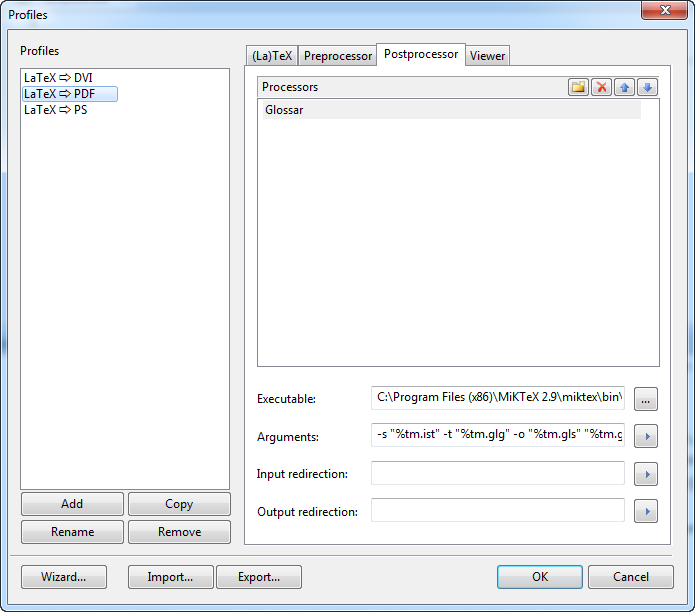
\includegraphics[scale=0.6]{images/profiles_glossar.png}
	\caption{Post-processing}
	\label{fig:postprocessing}
\end{figure}


\section{Bibliography}
\label{sec:instructions_bibliography}

To compile a bibliography\index{bibliography} one must resort to \gls{BibTeX}. The folder \texttt{database} includes a \texttt{.bib} file with various database entries. How the entries are to be compiled, can be taken from various sources of the Internet or books. The entries in the database will only be written to the directory of the document when the source is actually cited in the text.

Under the following addresses further explanations are found in order to compile the database and its use:

\begin{itemize}
	\item \url{http://en.wikipedia.org/wiki/BibTeX}
	\item \url{http://www.bibtex.org/}
\end{itemize}



\chapter{Test of type area}
\label{chap:typeareatest}

Far far away, behind the word mountains, far from the countries Vokalia and Consonantia, there live the blind texts. Separated they live in Bookmarksgrove right at the coast of the Semantics, a large language ocean. A small river named Duden flows by their place and supplies it with the necessary regelialia. It is a paradisematic country, in which roasted parts of sentences fly into your mouth. Even the all-powerful Pointing has no control about the blind texts it is an almost unorthographic life One day however a small line of blind text by the name of Lorem Ipsum decided to leave for the far World of Grammar. 

\section{The Big Oxmox}
\label{sec:typeareatest_ombox}

The Big Oxmox advised her not to do so, because there were thousands of bad Commas, wild Question Marks and devious Semikoli, but the Little Blind Text didn’t listen. She packed her seven versalia, put her initial into the belt and made herself on the way. When she reached the first hills of the Italic Mountains, she had a last view back on the skyline of her hometown Bookmarksgrove, the headline of Alphabet Village and the subline of her own road, the Line Lane. Pityful a rethoric question ran over her cheek, then she continued her way. On her way she met a copy.

\begin{equation}
	\mathcal{N}(x \mid \mathbold{\mu}, \mathbold{\Sigma}) = \frac{1}{(2\pi)^{D/2}} \frac{1}{|\mathbold{\Sigma}|^{(1/2)}} \exp \left( -\frac{1}{2}(x-\mathbold{\mu})^{T}\mathbold{\Sigma}^{-1}(x-\mathbold{\mu}) \right)
\end{equation}

The copy warned the Little Blind Text, that where it came from it would have been rewritten a thousand times and everything that was left from its origin would be the word "and" and the Little Blind Text should turn around and return to its own, safe country. But nothing the copy said could convince her and so it didn’t take long until a few insidious Copy Writers ambushed her, made her drunk with Longe and Parole and dragged her into their agency, where they abused her for their projects again and again. And if she hasn’t been rewritten, then they are still using her.

\section{Type dummy text}
\label{sec:typeareatest_typedummytext}

This is a typo dummy text. On it you can see if all the letters there are and how they look. Sometimes one uses words like Hamburgefonts, Rafgenduks or Handgloves to test fonts. Sometimes phrases that contain all letters of the alphabet - one calls these sets "pangrams".

Well known is this: The quick brown fox jumps over the lazy old dog. Often in type dummy texts also foreign-language sentence parts are installed (AVAIL\textsuperscript{\texttrademark} and Wefox\textsuperscript{\textregistered} are testing aussi la Kerning) to test the effect in other languages. In Latin, for example, almost every font looks good.

\subsection{Demonstrandum}
\label{subsec:satzspiegeltest_typoblindtext_demonstrandum}

Quod erat demonstrandum. Seit 1975 fehlen in den meisten Testtexten die Zahlen, weswegen nach TypoGb. 204 \S ab dem Jahr 2034 Zahlen in 86 der Texte zur Pflicht werden. Nichteinhaltung wird mit bis zu 245 \texteuro oder 368\$ bestraft. Genauso wichtig in sind mittlerweile auch \^A\c{c}c\`e\~nt\"e, die in neueren Schriften aber fast immer enthalten sind. Ein wichtiges aber schwierig zu integrierendes Feld sind OpenType-Funktionalit\"aten. Je nach Software und Voreinstellungen k\"onnen eingebaute Kapit\"alchen, Kerning oder Ligaturen (sehr pfiffig) nicht richtig dargestellt werden.

\subsubsection{Subsubsection}

This is a typo dummy text. On it you can see if all the letters there are and how they look. Sometimes one uses words like Hamburgefonts, Rafgenduks or Handgloves to test fonts. Sometimes phrases that contain all letters of the alphabet - one calls these sets "pangrams". 

\subsubsection{Subsubsection}

Well known is this: The quick brown fox jumps over the lazy old dog. Often in type dummy texts also foreign-language sentence parts are installed (AVAIL\textsuperscript{\texttrademark} and Wefox\textsuperscript{\textregistered} are testing aussi la Kerning) to test the effect in other languages. In Latin, for example, almost every font looks good. Quod erat demonstrandum.

\section{Webstandards}
\label{sec:satzspiegeltest_webstandards}

Everywhere the same old story. The layout is complete, the text is slow in coming. This layout is now not naked in space and small and empty occurs, I help out: the dummy text. Created exactly for this purpose, always in the shadow of my big brother "Lorem Ipsum", I look forward every time you read a few lines. Because esse est percipi - being is to be perceived.

And now because you already have the goodness to accompany me a few more sentences long, I would like to take this opportunity to serve you not only as a stopgap, but to point out something that is going to be perceived as deserved: Web viz. See Web standards are the rules that build on the websites. So there are rules for HTML, CSS, JavaScript or XML, words that you might have heard of your developers. These standards ensure that all parties the maximum benefit from a website.

\begin{figure}[H]
	\centering
		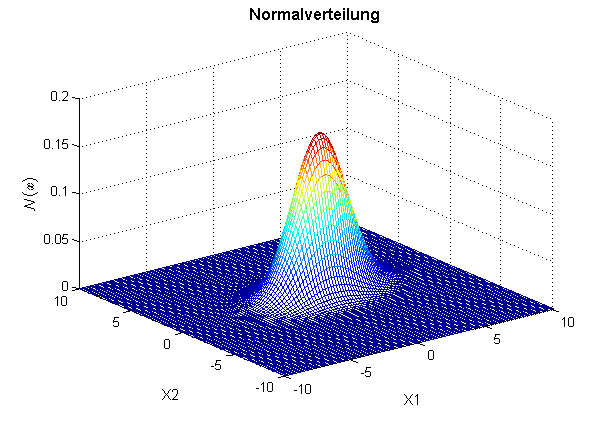
\includegraphics[scale=0.7]{images/multivariate_gauss.png}
	\caption{Normal distribution}
	\label{fig:normal_distribution}
\end{figure}

In contrast to previous websites we no longer need, for example, two different sites for the program Internet Explorer and another browser. It extends a page that - properly applied - both works on different browsers on the net, but just as good for printing or display on a cell phone is. Mind: A site for all formats. What a relief. Standards save time provide for the development costs and ensure that web pages can be easier to maintain later. Of course, only if everyone adheres to these standards.

\chapter{Conclusion / Results}
\label{chap:conclusions}
Overall the process of the preliminary study did not work out as expected. On one hand the technical requirements for the programming environment caused way more problems than expected and on the other hand, the time planning and focus of the author did get out of hand. The combination of these two issues caused major time and motivation problems. Therefore the result of the preliminary study is not satisfying for the author in accordance to the initial expectation.
Nevertheless, working on this project is very interesting and challenging, which means that the will to continue this project is unbroken.

Content wise there should have been a bigger accomplishment according the time given and the massive amount of time invested. After many hours of literature review, a sobering low amount of portable possibilities has been found. This leads to the conclusion that the way of research has to be adapted in order to find suitable solution for the existing issues.
Due to the adaption of the initial plan and the exchange with the experts, a realistic approach has been defined. Under consideration of all these factors, the best possible result is now provided.

The most important learning for the work on the milestones is to keep an strong focus on the actual tasks combined with a good and mindful time management. Also the exchange with other students and the experts shall be kept alive to benefit of the given knowledge. Help shall be searched at a earlier point of time, which does not mean, not to try to fix problems by the authors own possibilities and serious tries.

The definition of the milestones provides a promising planning of the Bachelor Thesis and seems to allow a good result for the main goal of the project. Needed Hardware and Software is mostly identified and methods to fulfill the requirements are described. 

An intense research of the topic and possible alternatives for occurred problems has been executed and leads to a knowledge which can be used and extended during the Bachelor Thesis.  

For the start of the Bachelor Thesis, only the learning will be taken into account and the disappointment is left behind. With great motivation and a strong will to perform well, the author is now looking forward to the realization of the milestones of the Bachelor Thesis. 

%---------------------------------------------------------------------------

% Selbst�ndigkeitserkl�rung
%---------------------------------------------------------------------------
\cleardoublepage
\phantomsection 
\addcontentsline{toc}{chapter}{Declaration of authorship}
\chapter*{Declaration of primary authorship}
\label{chap:declaration_authorship}

\vspace*{10mm} 

I hereby confirm that I have written this thesis independently and without using other sources and resources than those specified in the bibliography. All text passages which were not written by me are marked as quotations and provided with the exact indication of its origin. 

\vspace{15mm}

\begin{tabbing}
xxxxxxxxxxxxxxxxxxxxxxxxxxxxxx\=xxxxxxxxxxxxxxxxxxxxxxxxxxxxxx\=xxxxxxxxxxxxxxxxxxxxxxxxxxxxxx\kill
Place, Date:		\> Biel, \versiondate \\ \\ 
Last Name, First Name:	\> Aeschlimann, Dario 	\>  \\ \\ \\ \\ 
Signature:	\> ......................................\> ...................................... \\
\end{tabbing}

%---------------------------------------------------------------------------

% Glossary
%---------------------------------------------------------------------------
\cleardoublepage
\phantomsection 
\addcontentsline{toc}{chapter}{Glossay}
%\renewcommand{\glossaryname}{Glossay}
\printglossary
%---------------------------------------------------------------------------

% Bibliography
%---------------------------------------------------------------------------
\cleardoublepage
\phantomsection 
\addcontentsline{toc}{chapter}{Bibliography}
\bibliographystyle{IEEEtranS}
\bibliography{database/bibliography}{}
%---------------------------------------------------------------------------

% Listings
%---------------------------------------------------------------------------
\cleardoublepage
\phantomsection 
\addcontentsline{toc}{chapter}{List of figures}
\listoffigures
\cleardoublepage
\phantomsection 
\addcontentsline{toc}{chapter}{List fo tables}
\listoftables
%---------------------------------------------------------------------------

% Index
%---------------------------------------------------------------------------
\cleardoublepage
\phantomsection 
\addcontentsline{toc}{chapter}{Index}
\printindex
%---------------------------------------------------------------------------

% Attachment:
%---------------------------------------------------------------------------
\appendix
\settocdepth{section}
\chapter*{APPENDICES}
\addcontentsline{toc}{chapter}{APPENDICES}

\begingroup\let\clearpage\relax
\chapter{Arbitrary Appendix}
\label{chap:appendix_arb}
\endgroup

The European languages are members of the same family. Their separate existence is a myth. For science, music, sport, etc, Europe uses the same vocabulary. The languages only differ in their grammar, their pronunciation and their most common words. Everyone realizes why a new common language would be desirable: one could refuse to pay expensive translators. To achieve this, it would be necessary to have uniform grammar, pronunciation and more common words. If several languages coalesce, the grammar of the resulting language is more simple and regular than that of the individual languages. The new common language will be more simple and regular than the existing European languages. It will be as simple as Occidental; in fact, it will be Occidental. 
\chapter{Additional Appendix}
\label{chap:appendix_B}

\section{Test 1}
To an English person, it will seem like simplified English, as a skeptical Cambridge friend of mine told me what Occidental is. The European languages are members of the same family. Their separate existence is a myth. For science, music, sport, etc, Europe uses the same vocabulary. The languages only differ in their grammar, their pronunciation and their most common words. Everyone realizes why a new common language would be desirable: one could refuse to pay expensive translators. To achieve this, it would be necessary to have uniform grammar, pronunciation and more common words. If several languages coalesce, the grammar of the resulting language is more simple and regular than that of the individual languages. The new common language will be more simple and regular than the existing European languages. 

\subsection{Environment}
It will be as simple as Occidental; in fact, it will be Occidental. To an English person, it will seem like simplified English, as a skeptical Cambridge friend of mine told me what Occidental is. The European languages are members of the same family. Their separate existence is a myth. For science, music, sport, etc, Europe uses the same vocabulary. The languages only differ in their grammar, their pronunciation and their most common words. Everyone realizes why a new common language would be desirable: one could refuse to pay expensive translators. To achieve this, it would be necessary to have uniform grammar, pronunciation and more common words.
\chapter{Content of CD-ROM}
\label{chap:appendix_CDROM}

Content of the enclosed CD-ROM, directory tree, etc.
%---------------------------------------------------------------------------

%---------------------------------------------------------------------------
\end{document}

